\section{SCD}
\thispagestyle{fancy}

Etter vi hadde valt dei blokkene vi ønskte var det naturleg å sette seg ned å planlegge korleis vi ønska å knytte desse blokkene opp i mot anlegget. 
Vi valte da å starte med å lage eit System Control Diagram (SCD) over anlegget. 
SCD er ein grafisk representasjon av anlegget, som visar komponentane i anlegget og deira funksjon, forbindelsar og struktur. 
IEC PAS 63131 standaren gir oss retningslinjene for utforming av diagrammet.


\begin{figure}[htbp]
    \centering
    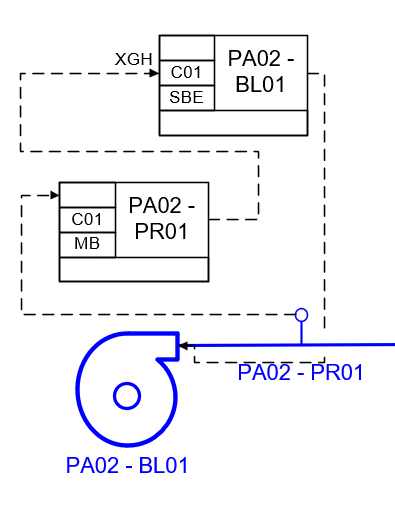
\includegraphics[width=0.35\textwidth]{Bilder/Visio_eksempel.png}
    \caption{Utsnitt frå SCD}\label{fig:SCD eksempel}    
\end{figure}


Første utkast av vårt SCD inneheldt koplingane frå komponentar til blokker og korleis forbindelsane imellom desse skulle fungere. 
Korleis dei forskjellige sekvensane skulle interagere med blokkene og komponentane våre var litt uklart for oss på detta stadiet,
så vi valde å gå vidare med å lage noko av programmet, slik at vi lettare kunne danne oss eit bilete av korleis vi ville løyse oppgåva.


\newpage